\documentclass{article}


% if you need to pass options to natbib, use, e.g.:
%     \PassOptionsToPackage{numbers, compress}{natbib}
% before loading neurips_2023

% ready for submission
\usepackage[final]{neurips_2023}
\usepackage{graphicx}
\usepackage{array}
\usepackage{amsmath}
\usepackage{subfigure}
\usepackage{titlesec}
\usepackage{float}
\usepackage{placeins}
\usepackage{adjustbox}
\usepackage[utf8]{inputenc} % allow utf-8 input
\usepackage[T1]{fontenc}    % use 8-bit T1 fonts
\usepackage{hyperref}       % hyperlinks
\usepackage{url}            % simple URL typesetting
\usepackage{booktabs}       % professional-quality tables
\usepackage{amsfonts}       % blackboard math symbols
\usepackage{nicefrac}       % compact symbols for 1/2, etc.
\usepackage{microtype}      % microtypography
\usepackage{xcolor}         % colors


\title{Semantic Segmentation of Images}

\author{
  Connor Gag \\
  \texttt{cgag@ucsd.edu} \\
  \And
  Shivangi Karwa \\
  \texttt{skarwa@ucsd.edu} \\
  \And
  Hansin Patwa \\
  \texttt{hpatwa@ucsd.edu} \\
  \And
  Max Yang \\ 
  \texttt{guy006@ucsd.edu}
}

% The \author macro works with any number of authors. There are two commands
% used to separate the names and addresses of multiple authors: \And and \AND.
%
% Using \And between authors leaves it to \LaTeX{} to determine where to break
% the lines. Using \AND forces a linebreak at that point. So, if \LaTeX{}
% puts 3 of 4 authors names on the first line, and the last on the second
% line, try using \AND instead of \And before the third author name.

\newcommand{\fix}{\marginpar{FIX}}
\newcommand{\new}{\marginpar{NEW}}


\begin{document}


\maketitle

\begin{abstract}
In this study, we explore the task of semantic segmentation using different Convolutional Neural Network architectures, specifically focusing on the PASCAL VOC-2012 dataset to classify objects at the pixel level, evaluating their performance using pixel accuracy and Intersection-over-Union (IoU) metrics. Our baseline model is a deep Fully Connected Convolutional Network trained with Xavier weight initialization and optimized using the Adam optimizer. The mean pixel accuracy is $73.77\%$, and the mean IoU is $0.0665$. To enhance the performance, we also try cosine annealing learning rate scheduling, data augmentation techniques (random cropping, flipping), and a weighted loss function to mitigate class imbalance. Additionally, we experiment with a custom architecture integrating dropout layers and transfer learning using ResNet-34. Results indicate that the ResNet-based model outperforms the baseline, with 0.833 pixel accuracy and 0.188 mean IoU. However, our custom architecture showed only marginal improvements over the baseline, suggesting a trade-off between overfitting prevention and information retention.
\end{abstract}

\section{Introduction}
Semantic segmentation is important in the AI field today. It enables machines to recognize and interpret the image at a pixel level by assigning a class label to every pixel in an image. This capability is essential for many applications, including but not limited to self-driving, disease detection, remote sensing, etc. 

The main goal of this project is to recognize objects from a number of visual object classes in realistic scenes. We build a Convolutional Neural Network to achieve the semantic segmentation task with the PASCAL VOC-2012 dataset, which has pixel-wise annotation. There are 21 categories in the dataset with 20 object categories and 1 background category.

There are two major metrics to measure how good a model is. The first one is the pixel accuracy, which is defined as:
\begin{eqnarray}
    \text{Percent correct predictions} =\frac{\text { total correct predictions }}{\text { total number of samples }}
\end{eqnarray}
The other metrics is called Intersection-Over-Union (IoU): The IoU is the area of overlap between the predicted segmentation and the ground truth divided by the area of union between the predicted segmentation and the ground truth:
\begin{eqnarray}
    \mathrm{IoU}=\frac{T P}{T P+F P+F N}
\end{eqnarray}
where TP, FP, and FN are the numbers of true positive, false positive, and false negative pixels. 
With these two metrics in hand, the goal of this project is to build a network to reach the accuracy and IoU as high as possible.


\section{Related Work}
The major part of the code is consistent with the course materials. We also follow the \cite{ronneberger_u-net_2015} U-Net architecture while adjusting this architecture to our specific problem.

We also used the ResNet structure found in \cite{he_deep_2015} to experiment and improve the result. Not only did we use the architecture of ResNet, we also used the weights using the pytorch ResNet library.

\section{Methods}\label{sec:method}

We’re using Xavier weight initialization as found in \cite{glorot2010understanding} and batch normalization. This is used to prevent the exploding and vanishing gradient problems. It also leads to quicker convergence.

Xavier weight initialization sets the weights of a layer to random values between the following values:

$\left(-\frac{\sqrt{6}}{\sqrt{n_{\text{in}} + n_{\text{out}}}}\right) \text{ and } \left( \frac{\sqrt{6}}{\sqrt{n_{\text{in}} + n_{\text{out}}}}\right)$

These random values fit into a uniform distribution. Lastly, another important aspect of our implementation is that we used the Adam gradient descent optimizer.

\subsection{Baseline}

In the baseline model, we built a fully connected deep convolutional neural network with the RELU activation function. The last layer has 21 out channels, signifying the number of categories we have. We did not apply a softmax or any activation function at the end of our forward function because the softmax is applied within the cross entropy loss function that we implemented. We used Xavier weight initialization as discussed in the Methods section. Our gradient descent optimizer was Adam.

Below is our architecture of the base FCN model:

\begin{table}[H]
  \centering
  \caption{Baseline Structure}
    \begin{tabular}{lcccccc}
    \toprule
    \multicolumn{1}{c}{Layers} & In channel & Out channel & Kernel Size & Stride & Padding & Dilation \\
    \midrule
    Convolutional Layer1 & 3     & 32    & 3     & 2     & 1     & 1 \\
    ReLu Layer &       &       &       &       &       &  \\
    Normalization Layer1 & 32    & 32    &       &       &       &  \\
    Convolutional Layer2 & 32    & 64    & 3     & 2     & 1     & 1 \\
    ReLu Layer &       &       &       &       &       &  \\
    Normalization Layer2 & 64    & 64    &       &       &       &  \\
    Convolutional Layer3 & 64    & 128   & 3     & 2     & 1     & 1 \\
    ReLu Layer &       &       &       &       &       &  \\
    Normalization Layer3 & 128   & 128   &       &       &       &  \\
    Convolutional Layer4 & 128   & 256   & 3     & 2     & 1     & 1 \\
    ReLu Layer &       &       &       &       &       &  \\
    Normalization Layer4 & 256   & 256   &       &       &       &  \\
    Convolutional Layer5 & 256   & 512   & 3     & 2     & 1     & 1 \\
    ReLu Layer &       &       &       &       &       &  \\
    Normalization Layer5 & 512   & 512   &       &       &       &  \\
    DeConvolutional Layer1 & 512   & 512   & 3     & 2     & 1     & 1 \\
    ReLu Layer &       &       &       &       &       &  \\
    Normalization Layer6 & 512   & 512   &       &       &       &  \\
    DeConvolutional Layer2 & 512   & 256   & 3     & 2     & 1     & 1 \\
    ReLu Layer &       &       &       &       &       &  \\
    Normalization Layer7 & 256   & 256   &       &       &       &  \\
    DeConvolutional Layer3 & 256   & 128   & 3     & 2     & 1     & 1 \\
    ReLu Layer &       &       &       &       &       &  \\
    Normalization Layer8 & 128   & 128   &       &       &       &  \\
    DeConvolutional Layer4 & 128   & 64    & 3     & 2     & 1     & 1 \\
    ReLu Layer &       &       &       &       &       &  \\
    Normalization Layer9 & 64    & 64    &       &       &       &  \\
    DeConvolutional Layer5 & 64    & 32    & 3     & 2     & 1     & 1 \\
    ReLu Layer &       &       &       &       &       &  \\
    Normalization Layer10 & 32    & 32    &       &       &       &  \\
    Convolutional Classifier & 32    & 21    & 1     &       &       &  \\
    \bottomrule
    \end{tabular}%
  \label{tab:baseline}%
\end{table}%

\subsection{Improvements over Baseline}

We made several key improvements to our model, including optimizing the learning rate schedule, applying data augmentations, and addressing class imbalances. These changes enhance generalization and robustness.

\subsubsection{Cosine Annealing} 

We utilized the cosine annealing learning rate scheduler to adjust the learning rate dynamically over the course of training epochs. This approach helped improve convergence by gradually reducing the learning rate, allowing the model to settle into a better minimum while avoiding sharp drops in performance. Using Cosine Annealing Scheduler, we were able to achieve IOU of $0.0662$ and pixel accuracy of $73.6\%$.

\subsubsection{Transformations} 
We randomly cropped $30\%$ of the images with the fraction of the original image area between 0.9 and 1, and the aspect ratio between $\frac{3}{4}$ and $\frac{4}{3}$. We also randomly flipped mirrors on $30\%$ of the pictures as well as the labels.

Below is an example of applying the image transformations to a sample image. We applied both a mirror flip and a random cropping to this image. However, the chose and transformations are not necessarily done on the same images. 30\% of the images are randomly chosen for flipping and 30\% are randomly chosen for cropping. Augmenting the data resuled in an IOU of $0.069$ and pixel accuracy of $73.71\%$.

\begin{figure}[H]
    \centering
    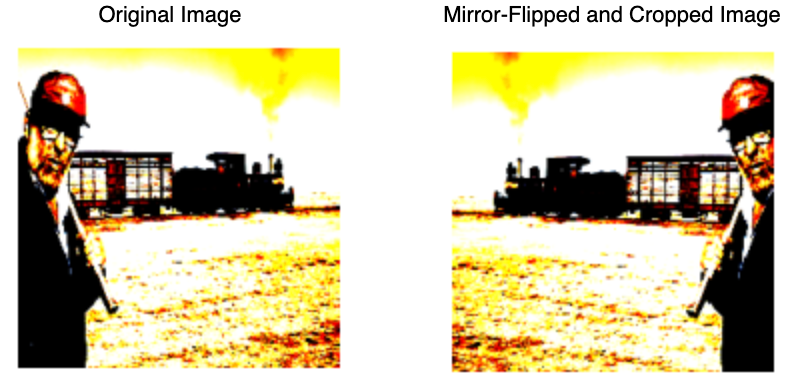
\includegraphics[width=0.8\linewidth]{augmentations_example.png}
\end{figure}

\subsubsection{Imbalance problem} 
 To deal with the class imbalance, we implemented the weighted loss function. To obtain the weights, we simply went through each of the training mask and count the number of pixels for each class. To get the class weights we take the inverse of those counts. To prevent division by 0 we add a very small number to each of the counts.

 By resolving the issue of class imbalance, we were able to achieve an IOU of $0.064$ and pixel accuracy of $74.14\%$.

\subsection{Experimentation}
\subsubsection{Custom Architecture}
We tried different architectures built on the baseline model. We add the dropout layers between the first block of convolutional and deconvolutional sections, which consists of convolutional and normalization layers, with different probabilities of an element to be zeroed. The reason why only adding dropout layers between the first block is to minimize the influence of dropping information. The probability within the convolutional section is set to 0.1, and the probability within the deconvolutional section is set to 0.15. During the experiment, we also followed the similar data augmentation we used above, including randomly cropping and flipping, and tried different learning rates with the Cosine Annealing schedule and class balancing. Table \ref{tab:custom} shows the architecture of our experimental network.
\begin{table}[H]
  \centering
  \caption{Experiment Structure}
  \adjustbox{max width=\textwidth}{
    \begin{tabular}{lccccccc}
    \toprule
    \multicolumn{1}{c}{Layers} & In channel & Out channel & Kernel Size & Padding & Stride & Dilation & Fraction of Zero \\
    \midrule
    Convolutional Layer1 & 3     & 32    & 3     & 2     & 1     & 1     &  \\
    ReLu Layer &       &       &       &       &       &       &  \\
    Normalization Layer1 & 32    & 32    &       &       &       &       &  \\
    Dropout Layer &       &       &       &       &       &       & 0.1 \\
    Convolutional Layer2 & 32    & 64    & 3     & 2     & 1     & 1     &  \\
    ReLu Layer &       &       &       &       &       &       &  \\
    Normalization Layer2 & 64    & 64    &       &       &       &       &  \\
    Convolutional Layer3 & 64    & 128   & 3     & 2     & 1     & 1     &  \\
    ReLu Layer &       &       &       &       &       &       &  \\
    Normalization Layer3 & 128   & 128   &       &       &       &       &  \\
    Convolutional Layer4 & 128   & 256   & 3     & 2     & 1     & 1     &  \\
    ReLu Layer &       &       &       &       &       &       &  \\
    Normalization Layer4 & 256   & 256   &       &       &       &       &  \\
    Convolutional Layer5 & 256   & 512   & 3     & 2     & 1     & 1     &  \\
    ReLu Layer &       &       &       &       &       &       &  \\
    Normalization Layer5 & 512   & 512   &       &       &       &       &  \\
    DeConvolutional Layer1 & 512   & 512   & 3     & 2     & 1     & 1     &  \\
    ReLu Layer &       &       &       &       &       &       &  \\
    Normalization Layer6 & 512   & 512   &       &       &       &       &  \\
    Dropout Layer &       &       &       &       &       &       & 0.15 \\
    DeConvolutional Layer2 & 512   & 256   & 3     & 2     & 1     & 1     &  \\
    ReLu Layer &       &       &       &       &       &       &  \\
    Normalization Layer7 & 256   & 256   &       &       &       &       &  \\
    DeConvolutional Layer3 & 256   & 128   & 3     & 2     & 1     & 1     &  \\
    ReLu Layer &       &       &       &       &       &       &  \\
    Normalization Layer8 & 128   & 128   &       &       &       &       &  \\
    DeConvolutional Layer4 & 128   & 64    & 3     & 2     & 1     & 1     &  \\
    ReLu Layer &       &       &       &       &       &       &  \\
    Normalization Layer9 & 64    & 64    &       &       &       &       &  \\
    DeConvolutional Layer5 & 64    & 32    & 3     & 2     & 1     & 1     &  \\
    ReLu Layer &       &       &       &       &       &       &  \\
    Normalization Layer10 & 32    & 32    &       &       &       &       &  \\
    Convolutional Classifier & 32    & 21    & 1     &       &       &       &  \\
    \bottomrule
    \end{tabular}%  
    }
  \label{tab:custom}%
\end{table}%

\begin{table}[H]
    \centering
    \begin{tabular}{l c}
        \toprule
        \textbf{Metric} & \textbf{Value} \\
        \midrule
        Test Loss & 0.9972 \\
        Test IoU & 0.1382 \\
        Test Pixel Accuracy & 0.7855 \\
        \bottomrule
    \end{tabular}
    \caption{Test Performance Metrics}
    \label{tab:test_metrics_2}
\end{table}


\subsubsection{Transfer Learning with ResNet} 

We implemented ResNet 34, as described in \cite{he_deep_2015}, by using the pytorch module and replacing the encoder of our current model. This encoder has 34 convolutional layers and we removed the last two and fit it onto our decoder. This included the architecture and weights from the model. We allowed the model to adjust the ResNet weights during training to fine tune it to our task. The decoder layer weights were still allowed to be adjusted during training. The result was an increase in training, validation, and test accuracy. We kept the Cosine Annealing, class balancing, and image augmentation settings from earlier.


\begin{table}[H]
  \centering
  \caption{ResNet Structure}
  \adjustbox{width=\textwidth}{
    \begin{tabular}{lcccccc}
    \toprule
    \multicolumn{1}{c}{Layers} & In channel & Out channel & Kernel Size & Stride & Padding & Dilation \\
    \midrule
    ResNet Encoder (Removed last 2 layers) & 3 & 512  &       &       &       & \\
    DeConvolutional Layer1 & 512   & 512   & 3     & 2     & 1     & 1 \\
    ReLu Layer &       &       &       &       &       &  \\
    Normalization Layer6 & 512   & 512   &       &       &       &  \\
    DeConvolutional Layer2 & 512   & 256   & 3     & 2     & 1     & 1 \\
    ReLu Layer &       &       &       &       &       &  \\
    Normalization Layer7 & 256   & 256   &       &       &       &  \\
    DeConvolutional Layer3 & 256   & 128   & 3     & 2     & 1     & 1 \\
    ReLu Layer &       &       &       &       &       &  \\
    Normalization Layer8 & 128   & 128   &       &       &       &  \\
    DeConvolutional Layer4 & 128   & 64    & 3     & 2     & 1     & 1 \\
    ReLu Layer &       &       &       &       &       &  \\
    Normalization Layer9 & 64    & 64    &       &       &       &  \\
    DeConvolutional Layer5 & 64    & 32    & 3     & 2     & 1     & 1 \\
    ReLu Layer &       &       &       &       &       &  \\
    Normalization Layer10 & 32    & 32    &       &       &       &  \\
    Convolutional Classifier & 32    & 21    & 1     &       &       &  \\
    \bottomrule
    \end{tabular}%
    }
  \label{tab:baseline}%
\end{table}%


\begin{table}[H]
    \centering
    \begin{tabular}{l c}
        \toprule
        \textbf{Metric} & \textbf{Value} \\
        \midrule
        Test Loss & 0.9150 \\
        Test IoU & 0.1875 \\
        Test Pixel Accuracy & 0.8329 \\
        \bottomrule
    \end{tabular}
    \caption{Test Performance Metrics}
    \label{tab:test_metrics}
\end{table}


\begin{figure}[H]
    \centering
    \begin{minipage}{0.5\linewidth}
        \centering
        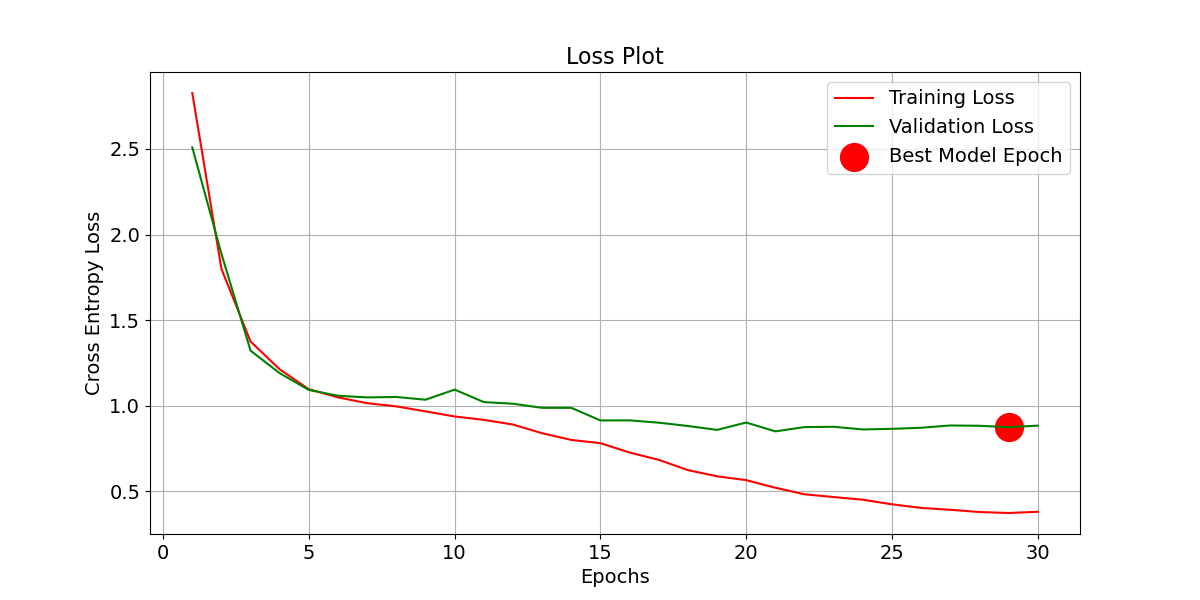
\includegraphics[width=\linewidth]{resnet_loss.png}
        \caption{Loss plot from ResNet training}
    \end{minipage}%
    \begin{minipage}{0.5\linewidth}
        \centering
        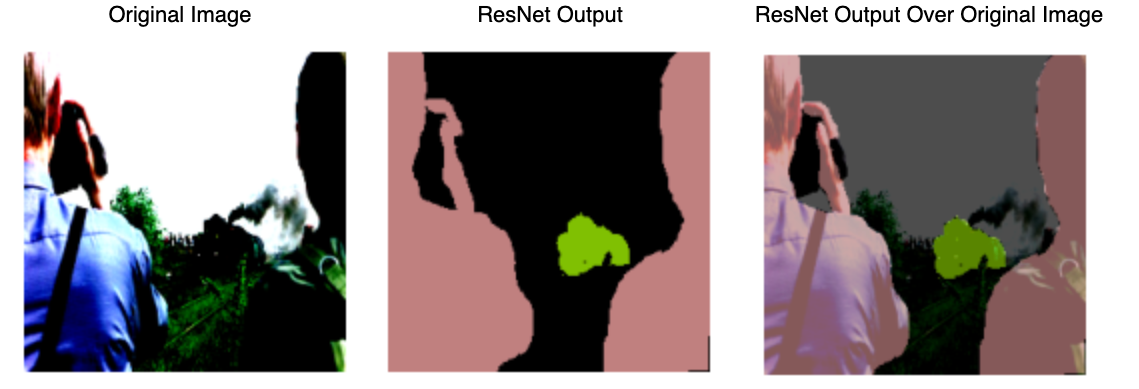
\includegraphics[width=\linewidth]{resnet_pictures.png}
        \caption{Sample output images from ResNet}
    \end{minipage}
\end{figure}



\newpage

\subsubsection{U Net}
\begin{table}[h]
\centering
\begin{tabular}{|c|c|c|c|c|c|c|}
\hline
\multicolumn{1}{|c|}{\textbf{Layers}} & \textbf{In Channels} & \textbf{Out Channels} & \textbf{Kernel Size} & \textbf{Stride} & \textbf{Padding} & \textbf{Dilation} \\
% \midrule
\hline
Conv1 (Encoder) & 3 & 64 & 3 & 1 & 1 & 1 \\
Conv2 (Encoder) & 64 & 128 & 3 & 1 & 1 & 1 \\
Conv3 (Encoder) & 128 & 256 & 3 & 1 & 1 & 1 \\
Conv4 (Encoder) & 256 & 512 & 3 & 1 & 1 & 1 \\
Conv5 (Bottleneck) & 512 & 1024 & 3 & 1 & 1 & 1 \\
UpConv1 (Decoder) & 1024 & 512 & 2x2 & 2 & 0 & 1 \\
Conv6 (Decoder) & 1024 & 512 & 3x3 & 1 & 1 & 1 \\
UpConv2 (Decoder) & 512 & 256 & 2x2 & 2 & 0 & 1 \\
Conv7 (Decoder) & 512 & 256 & 3x3 & 1 & 1 & 1 \\
UpConv3 (Decoder) & 256 & 128 & 2x2 & 2 & 0 & 1 \\
Conv8 (Decoder) & 256 & 128 & 3x3 & 1 & 1 & 1 \\
UpConv4 (Decoder) & 128 & 64 & 2x2 & 2 & 0 & 1 \\
Conv9 (Decoder) & 128 & 64 & 3x3 & 1 & 1 & 1 \\
Convolutional Classifier & 64 & n\_class & 1x1 & - & - & - \\
\hline
\end{tabular}
\caption{Layer-wise Description of U-Net Model}
\label{tab:network_layers}
\end{table}
\textbf{Note:} Each conv layer represents 2 conv layers which are represented as follows. The in channels and out channels depend on where they are in the network.

\begin{table}[H]
\begin{tabular}{|c|c|c|c|c|c|c|}
\hline
\multicolumn{1}{|c|}{\textbf{Layers}} & \textbf{In Channels} & \textbf{Out Channels} & \textbf{Kernel Size} & \textbf{Stride} & \textbf{Padding} & \textbf{Dilation} \\
\hline
Conv & input & output & 3 & 1 & 1 & 1 \\
BatchNorm  & output & output & - & - & - & - \\
Conv & output & output & 3 & 1 & 1 & 1 \\
BatchNorm  & output & output & - & - & - & - \\

\hline
\end{tabular}
\end{table}

We used the standard UNET implementation as directed in the paper with a slight modification of introducing batch norm. All input and output chaneles were maintained as directed in the UNET paper. All the activations were relu, except for the classifier layer having no activation. Batch norm brings regularization to the model. Below are the results - 

\begin{figure}[H]
    \centering
    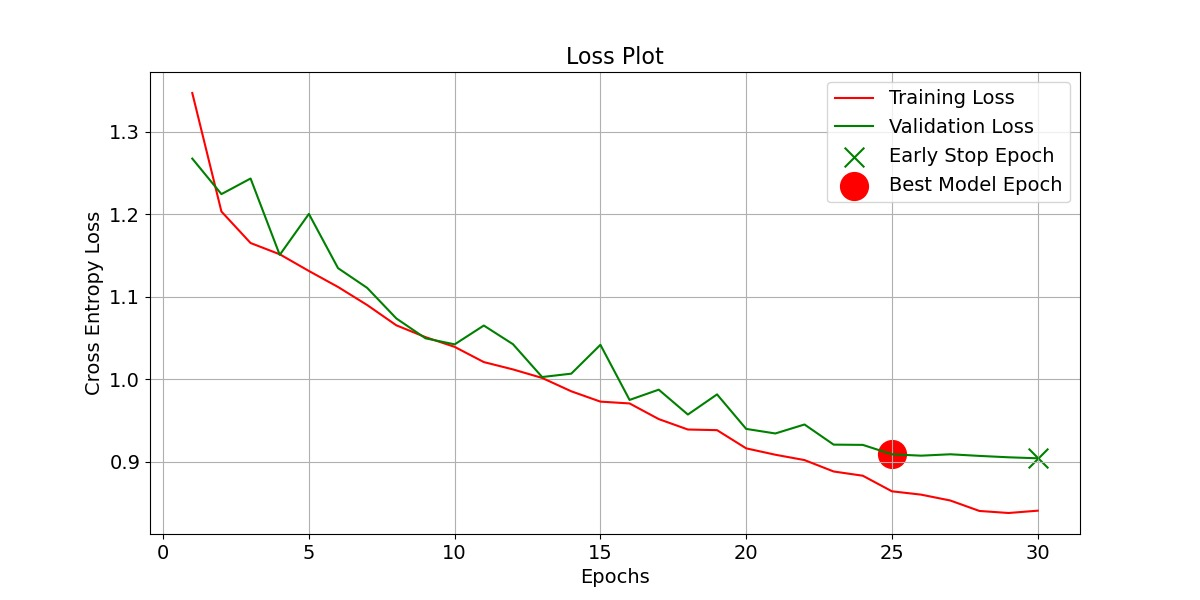
\includegraphics[width=0.8\linewidth]{unet.jpeg}
\end{figure}


\begin{table}[H]
    \centering
    \begin{tabular}{l c}
        \toprule
        \textbf{Metric} & \textbf{Value} \\
        \midrule
        Test Loss & 0.930 \\
        Test IoU & 0.083 \\
        Test Pixel Accuracy & 75.6\% \\
        \bottomrule
    \end{tabular}
    \caption{Test Performance Metrics}
    \label{tab:test_metrics}
\end{table}

\section{Results}

\begin{table}[H]
\centering
\begin{tabular}{|c|c|c|}
\hline
\textbf{Architecture} & \textbf{Pixel Accuracy} & \textbf{Average IoU} \\
\hline
Baseline Model & 73.77\% & 0.0665 \\
\hline
Cosine Annealing LR Scheduler & 73.6\% & 0.0662 \\
\hline
Image Augmentations & 73.71\% & 0.069 \\
\hline
Weighted Loss  & 74.14\% & 0.064 \\
\hline
\end{tabular}
\caption{Performance for Models on test sets (Pixel Accuracy and Average IoU)}
\label{tab:performance_metrics}
\end{table}


\begin{table}[H]
\centering
\begin{tabular}{|c|c|}
\hline
\textbf{Architecture} & \textbf{Image} \\
\hline
Baseline Model & 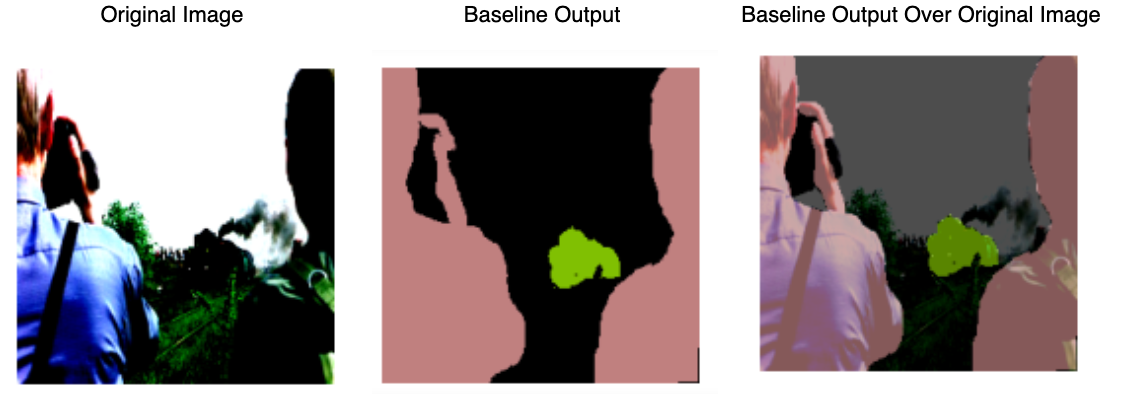
\includegraphics[width=0.6\textwidth]{baseline_images.png} \\
\hline
Cosine Annealing LR Scheduler & 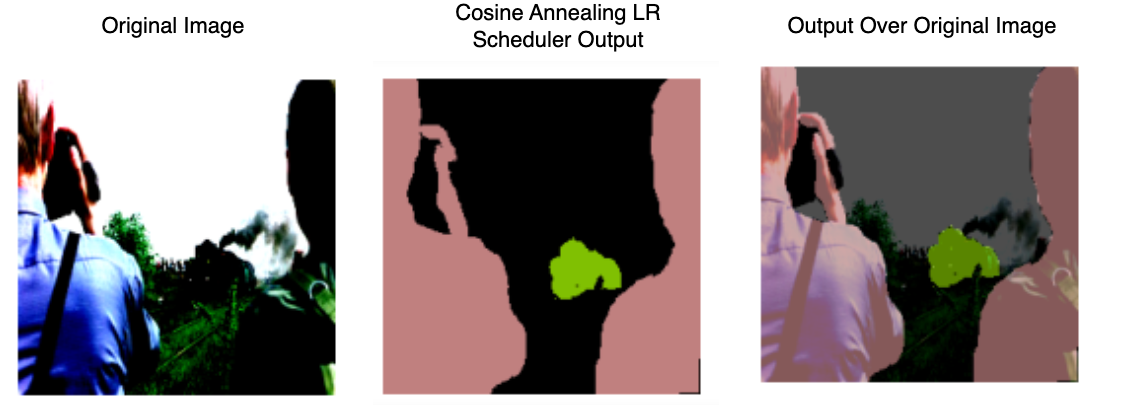
\includegraphics[width=0.6\textwidth]{annealing_pictures.png} \\
\hline
Image Augmentations & 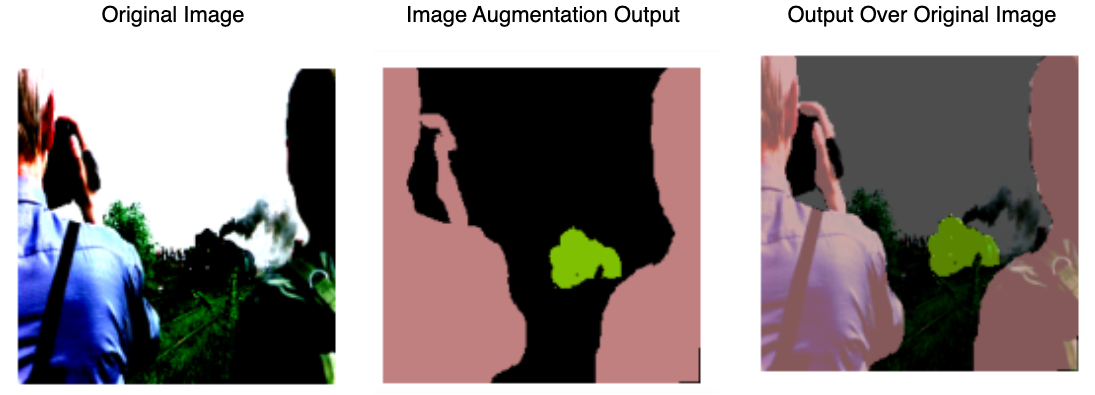
\includegraphics[width=0.6\textwidth]{augmentation_pictures.png} \\
\hline
Weighted Loss  & 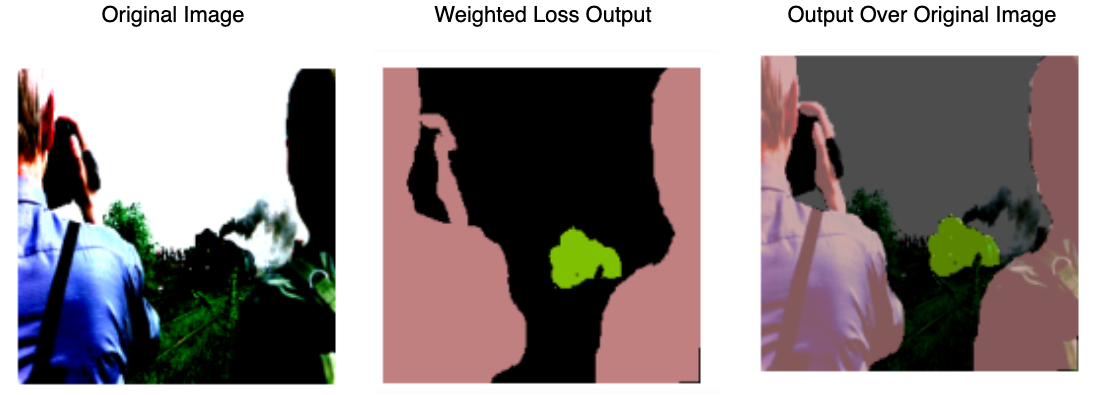
\includegraphics[width=0.6\textwidth]{weighted_loss_images.png} \\
\hline
\end{tabular}
\caption{Architecture and Image Visualizations for Models}
\label{tab:architecture_images}
\end{table}


\begin{table}[H]
\label{tab:results}
\centering
\begin{tabular}{|c|c|}
\hline
\textbf{Architecture} & \textbf{Loss} \\
\hline
Baseline Model & 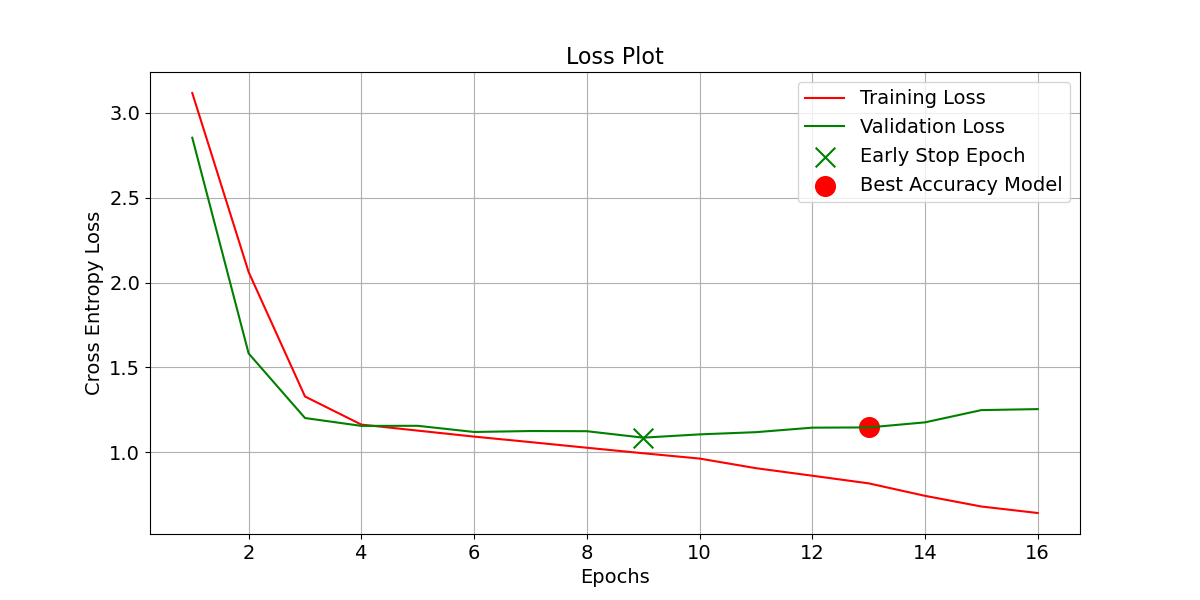
\includegraphics[width=0.6\textwidth]{loss_basic_fcn.png}\\
\hline
Cosine Annealing LR Scheduler & 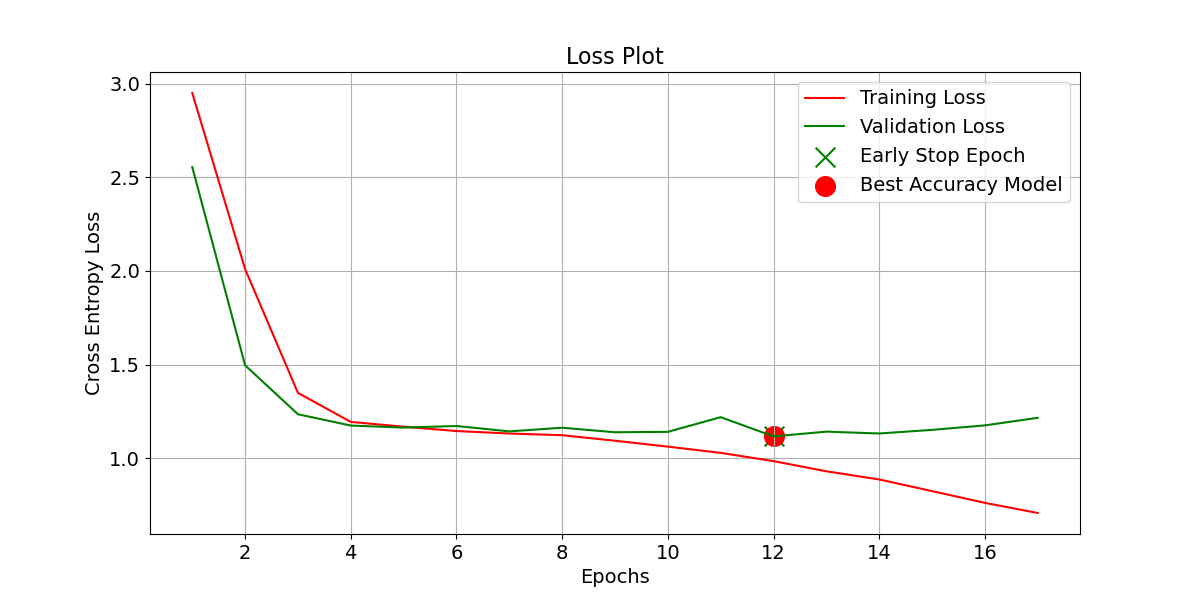
\includegraphics[width=0.6\textwidth]{cosine_plot.png} \\
\hline
Image Augmentations & 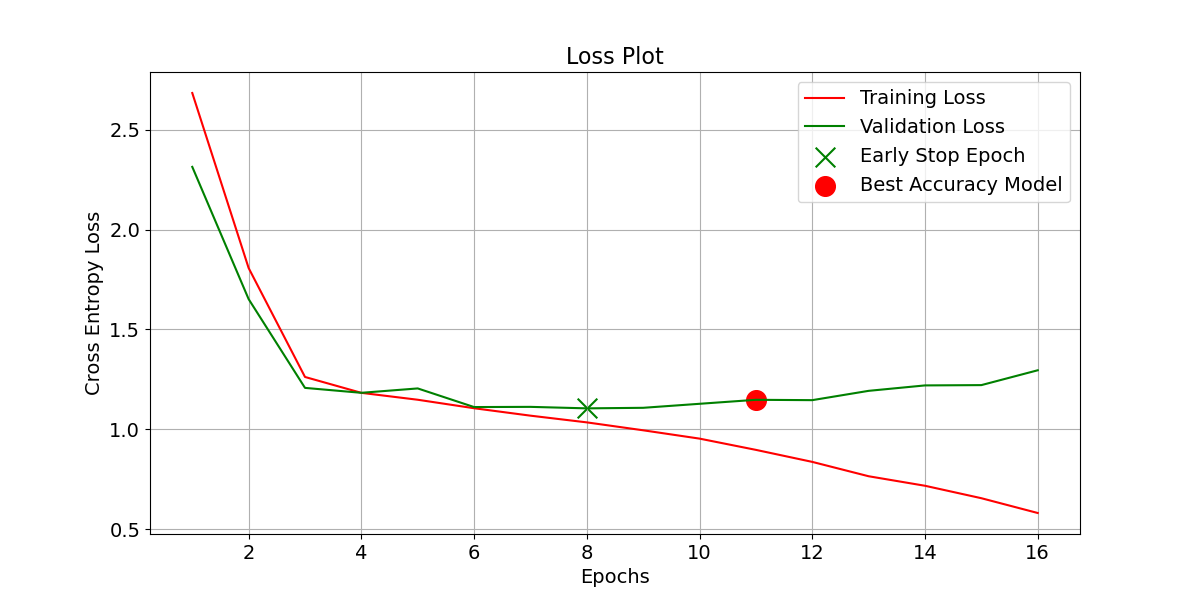
\includegraphics[width=0.6\textwidth]{loss_augment.png} \\
\hline
Weighted Loss  & 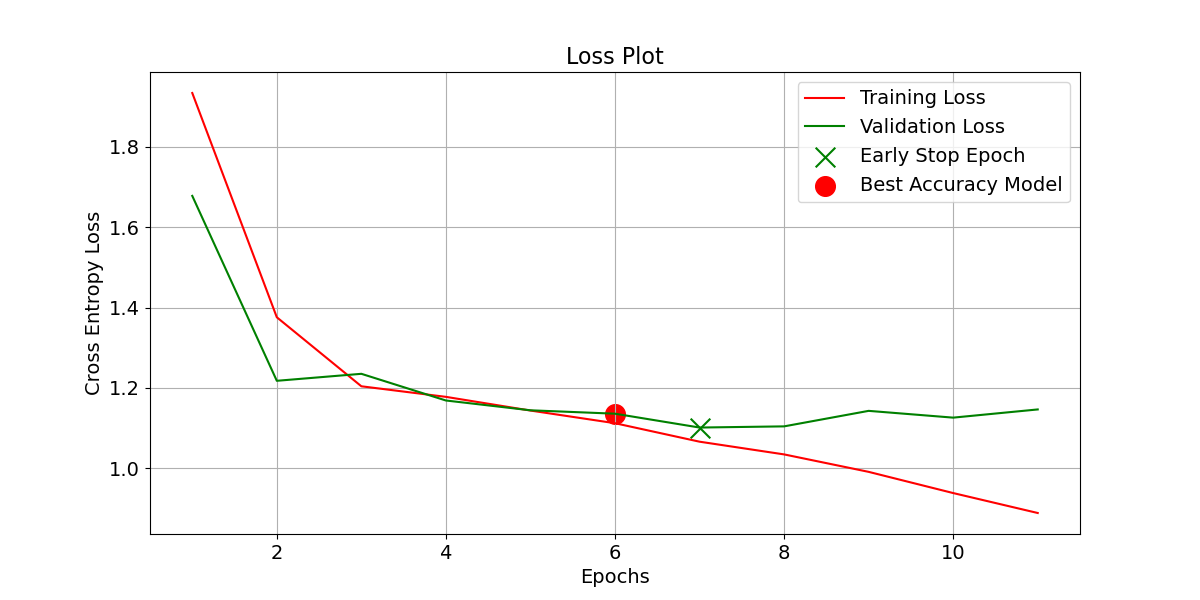
\includegraphics[width=0.6\textwidth]{class_loss.png} \\
\hline
\end{tabular}
\caption{Architecture and Training/Validation Loss for Models}
\label{tab:architecture_loss}
\end{table}


\subsection{Discussion on Baseline Model}

The baseline model used was a Fully Convolutional Network (FCN) trained on the VOC dataset with cross-entropy loss. This model provided a foundation for evaluating improvements and comparing other architectures. The FCN effectively captured spatial context through convolutional layers, which is important for semantic segmentation.The model showed some drawbacks, such as losing spatial details due to downsampling in deeper layers, slower convergence, and limited generalization.

The baseline model achieved a mean Intersection over Union (mIoU) of $0.066$. From the loss plot in \ref{tab:results}, the training loss consistently decreased, but the validation loss plateaued early, indicating overfitting after epoch 6, which is marked as the "Early Stop Epoch" (green cross). The best accuracy model (red circle) occurred at epoch 13, where validation loss was slightly lower. This divergence between training and validation losses shows that the model struggled with generalization due to insufficient regularization or data augmentation.

Overall, the baseline model performed reasonably well but had room for improvement in handling class imbalances and preventing overfitting. These results provide a benchmark for comparing the improved baseline and other architectures.


\subsection{Discussion on Improving Baseline Model}

The first improvement we made was adding a learning rate scheduler, cosine anealing. As we can see in the results there is hardly any improvement. but from the plot we can see that the training loss was a little lower. After this we implemented data augmentation, the 2 augmentations we employed were image cropping and flipping. This did result in model improvements having both better pixel accuracy and higher average IoU.  After this we implemented weighted loss to combat class imbalance this made a good improvement in our model taking the pixel accuracy to 77.9 having the most impact on the model. 

As we can see from the results section, the improvements that we implemented were necessary but not integral to the larger gains in accuracy that we saw. This point is shown by looking at the masks that were produced for all of the baseline improvements. All of the masks look about the same because the accuracies are very similar. The graphs of the loss functions all look relatively similar as well, where early stopping came into play as our model began to overfit around the 12th epoch.

\subsection{Discussion on Experimentation}

In our customized architecture, adding the dropout layers between different blocks is supposed to improve the overfitting problem. According to our experimental result, the pixel accuracy and average IoU are similar to the baseline model. This could be because of the trade-off between the benefit of improving overfitting and the loss of throwing information.

Our ResNet model performed quite well compared to our baseline model and other experiments. We used our other model enhancements such as cosine annealing, class balancer, and image augmentations as well. Using the pre-trained weights from ResNet 34 resulted in about a 4\% increase in the test accuracy. One thing to note is that allowing the ResNet weights to be changed during training improved the model's performance because it allowed back propagation to slightly fit ResNet's weights to our problem. 

UNET model did not perform as well as the other models. Though it did perform better then the baseline model. The main observations were that majority of the learning was completed in very early epochs, no change seemed to affect that even adaptive learning rates did not improve the accuracy by much. Adding batch norm to the layers did help to improve the model a little. We also maintained the weighted loss and image augmentation as removing them reduced the model performance. The model did manage to achieve a test pixel accuracy of 75.6\%. We can see from the graph that while the train loss curve was smooth the validation had a lot of changes.

\bibliographystyle{apalike}
\bibliography{PS2}
\end{document}